\chapter{Background and Related Work}
\label{chapter:Theoretical Framework and Related Work}



This chapter provides an overview of the theoretical framework and the relevant literature required for this master thesis. In Section \ref{section:Reinforcement Learning}, the basics of reinforcement learning are presented, a theoretical background that is necessary for later better understanding imitation learning and the terms on-policy and off-policy. In Section \ref{section:Imitation Learning}, after explaining what is imitation learning, several IL algorithms are classified according to our proposed definitions of on-policy and off-policy imitation learning. Lastly, Section \ref{section:Corrective Imitation Learning} focuses on D-COACH, the corrective imitation learning algorithm that will be the base of our proposed new framework.




\section{Reinforcement Learning}
\label{section:Reinforcement Learning}

Reinforcement learning is a branch of machine learning where an agent interacts with an environment in a trial-and-error manner with the objective of finding which of the actions it can take will maximize a numerical reward signal \cite{Sutton:1998}. Reinforcement learning makes use of Markov decision processes (MDP) a framework for sequential decision making problems defined by the tuple of sets $(\mathcal{S}, \mathcal{A}, \mathcal{P}, \mathcal{R})$, see Figure \ref{fig:reinforcement_learning}. At time step $t$, the agent finds itself at state $s_t \in \mathcal{S}$ and performs an action $a_t \in \mathcal{A}(s)$ on the environment following a policy $\pi: \mathcal{S} \rightarrow \mathcal{A}$. Then, and as a result of the transition function $\mathcal{P}$, the environment evolves to the next state $s_{t+1}$ where the agent receives a reward $r_{t+1} \in \mathcal{R}$. 

\begin{figure}[H]
    \centering
    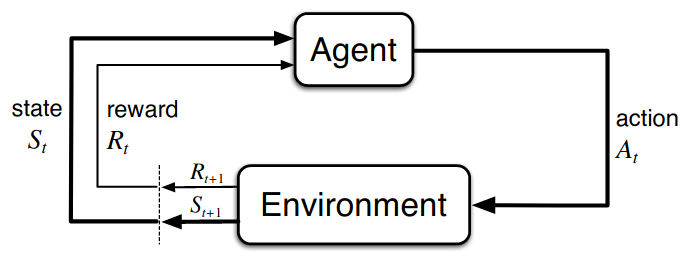
\includegraphics[width=.7\textwidth]{figures/reinforcement_learning.png}
    \caption{Interaction between the agent and the environment in reinforcement learning \cite{Sutton:1998}.}
    \label{fig:reinforcement_learning}
\end{figure}

% As the learning process continues, the agent and the environment produce a sequence or \textit{trajectory $\tau$} of states, actions and rewards:


% \begin{equation}
% \tau = s_0, a_0, r_1,s_1, a_1, r_2,s_2, a_2, r_3, ...
% \label{eq:transition}
% \end{equation}







MDPs satisfy the \textit{Markov property} that says that for a sequence of states $s_0, s_1, ..., s_t$, at any time $t$, the next state $s_{t+1}$ only depends on the current state $s_t$ \cite{Osa:2018}. A state, $s$, is a sufficient summary of what is going on in the environment and when it is possible to access all this sufficient information, the environment is said to be \textit{fully observable}. At every time step, the agent perceives an \textit{observation} that is a consequence of the state of the environment at that moment. Sometimes, just from the available observation, it is not possible to extract the state underneath and then, the environment is said to be \textit{partially observable}. The goal of the agent is to select the actions that will maximize the expected discounted return $G_t$ after $k$ time steps, see Equation \eqref{eq:expected-discounted-return}.
\begin{equation}
G_t = R_{t+1} + \gamma R_{t+2} + \gamma^2 R_{t+3} +... = \sum_{k=0}^{\infty} \gamma ^k R_{t+k+1}
\label{eq:expected-discounted-return}
\end{equation}




In previous Equation \eqref{eq:expected-discounted-return}, $\gamma$ is the \textit{discount rate}, a parameter in the range $0 \leq \gamma \leq 1$ that represents the value that future rewards have at the current time step $t$. At each time step, the environment sends a \textit{reward signal} to the agent that indicates how well the agent is performing in the \textit{immediate} sense. On the other hand, the \textit{value} of a state indicates how desirable is a state in the \textit{long-run}. In other words, the value of a state, $v_\pi \left(s\right) $, is the expected discounted return $G_t$ that an agent will receive over the future if it starts interacting at that state $s$ and continues following its policy $\pi$. This is captured by the \textit{value function} shown in Equation \eqref{eq:value-function}:






\begin{equation}
v_\pi \left(s\right) = E_\pi \left[G_{t}\mid S_{t}=s\right]
\label{eq:value-function}
\end{equation}



Similarly, the \textit{action-value function} or \textit{Q-function}, denoted as $q_\pi$ and shown in Equation \eqref{eq:q-function}, tells us how good it is for the agent to take an action at a given state while following a policy $\pi$. The output of the Q-function for any given state-action pair is called the \textit{Q-value}. 

\begin{equation}
q_\pi \left( s,a \right) = E_\pi \left[ G_{t}\mid S_{t}=s,A_{t}=a \right] 
\label{eq:q-function}
\end{equation}




When a reinforcement learning agent starts learning in an unknown environment it has to \textit{explore} new states to discover where the best rewards are. At the same time it has to \textit{exploit} what it already knows to choose the best actions. This is known as the \textit{exploration-exploitation }dilemma and it is a key challenge in reinforcement learning \cite{Sutton:1998}.




\subsection{On-policy and Off-policy Reinforcement Learning}
\label{subsection:on and off-policy Reinforcement Learning}

As presented in Chapter \ref{chapter:introduction}, the objective of this thesis is to develop an extension of the D-COACH method that is able to learn by replaying old corrections. We consider that there is a simile between this challenge and the concepts on-policy and off-policy in reinforcement learning given that, \say{when learning by experience replay, it is necessary to learn off-policy} \cite{Atari-RL}.

% One of the objectives of this literature review is to establish a clear definition of the concepts on-policy and off-policy in the field of imitation learning. Before that, in this section we will explain their meaning of these terms in reinforcement learning, a field where they are widely used and well known. To the best of our knowledge, the first mention of the terms on-policy and off-policy in reinforcement learning is found in the book \textit{Introduction to Reinforcement Learning} by \cite{Sutton:1998}.

According to Sutton and Barto, off-policy methods use two policies: They evaluate or improve a policy, the target policy, while using a different policy to generate the data, the behavior policy. In this case, we say that learning is from data \quotes{off} the target policy, and the overall process is termed off-policy learning \cite{Sutton:1998}. On the other hand, on-policy methods use a single policy, the same policy that is evaluated or improved, is the one used to generate behavior. 
To better understand the terms, we are going to briefly explore two popular RL algorithms, Q-Learning \cite{Watkins:1989} and SARSA \cite{Rummery+Niranjan:1994} to understand what makes the former off-policy and the later on-policy.


% SARSA and Q-learning are Temporal Difference (TD) algorithms that update the knowledge of the agent at every time step by bootstrapping which means that the update is partly based on other learned estimates, without waiting to know the final outcome \cite{Sutton:1998}. Equation \eqref{eq:TD} shows the general update rule of these TD methods \cite{TD:equation:2019}, here \textit{step size} is equivalent to learning rate.


% \begin{equation}
% \text{New estimate } \leftarrow \text{ Old estimate }+ \text{ Step size }* \left[\text{ Target - Old estimate} \right]
% \label{eq:TD}
% \end{equation}


% The SARSA, unlike Q-learning, the policy that SARSA evaluates, is the same with which it generates samples. Equation \eqref{eq:SARSA} shows its update rule.

In SARSA the agent starts at state $s_t$ and chooses an action $a_t$ according to its policy $\pi(s_t, a_t)$. Then, it observes the reward $r_t$ and the next state $s_{t+1}$ where it chooses the next action $a_{t+1}$ again according to its policy $\pi(s_{t+1}, a_{t+1})$. At this point it has all the required information to apply the update rule showed in Equation \eqref{eq:SARSA}.

\begin{equation}
Q^{\text{new}}(s_t, a_t)  \leftarrow Q(s_t, a_t) + \alpha \left[R+ \gamma  Q(s_{t+1}, a_{t+1}) - Q(s_t, a_t)\right]
\label{eq:SARSA}
\end{equation}

% Q-learning is similar to SARSA with the difference that for the \textit{update step}, see equation Equation \eqref{eq:Q-learning}, it takes the maximum of all possible actions.  This is the reason why it is called off-policy, because for the update, it ignores the policy $\pi$ that was used to take action $a_t$ at state $s_t$. 

Q-learning is similar to SARSA with the difference that for the \textit{update step}, it uses a \textit{greedy} policy that chooses the actions that yields the highest estimated Q-value, see Equation \eqref{eq:Q-learning}).  This is the reason why it is called off-policy, because, for the update, it ignores the policy $\pi$ that was used to take action $a_t$ at state $s_t$. 

%(see the \textit{max} in Equation \eqref{eq:Q-learning})
% But you then perform the actual next action based on your current policy

% Q-Learning   ..... Equation \eqref{eq:Q-learning} shows the update rule for this method where $s_t$ and $a_t$ are the state and action at time step $t$, $R$ is the reward obtained for taking $a_t$ at state $s_t$, $\alpha$ is the step size or learning rate and $\gamma$ is  the discount rate. The term $\max_{a} Q(s_{t+1}, a)$ represents  the best estimated value for the next state $s_{t+1}$ and it is independent of the policy being followed.

\begin{equation}
Q^{\text{new}}(s_t, a_t)  \leftarrow Q(s_t, a_t) + \alpha \left[ R  + \gamma {\max_{a} Q(s_{t+1}, a)} - Q(s_t, a_t)\right]
\label{eq:Q-learning}
\end{equation}





% When comparing both updating rules in Equations \eqref{eq:Q-learning} and \ref{eq:SARSA}, we can see that in Q-learning the agent learns the optimal policy by using a greedy policy when updating the Q-value (see the \textit{max} in Equation \eqref{eq:Q-learning}). This is what makes Q-learning off-policy, 



The fact that Q-learning uses a policy for generating behaviour different from the greedy policy with which it updates the Q-values is the key to understand why Q-learning can use experience replay, see Section \ref{subsection:Experience Replay}.


% The fact that Q-learning uses a policy for generating behaviour different from the greedy policy with which it updates the Q-values is what makes it suitable for also being able to 

% . This is key to understand why Q-learning can make use of the experience replay technique as we will see in Section \ref{subsection:Experience Replay}.

% On the other hand, SARSA





\subsection{Online and Offline Reinforcement Learning} 
\label{subsection:Online and Offline}

Reinforcement learning algorithms can also be classified according to how data is collected. Traditional RL algorithms are online frameworks where the agent iteratively interacts in its environment, collecting experience to update its policy. Online methods can be on-policy or off-policy depending on whether the data is exclusively gathered by the current policy or not, see the previous section.
The online approach works well in simulated environments however, for real-world settings, online learning is impractical because the agent still needs to collect a diverse and large dataset. 

Offline reinforcement learning, addresses the aforementioned problem. The key idea is that using only previously collected data, the agent has to learn the best possible policy without additional online data collection \cite{Offline-RL-Levine:2020}. With this offline framework, it is possible to apply RL to real-world domains like robotics where the agent, the robot, could easily get damaged while collecting data iteratively in an online manner. The downside of offline learning resides in collecting a suitable dataset for training, which for many real-world applications, can be very expensive to acquire \cite{collecting_data_for_offline_learning}.


\subsection{Experience Replay}
\label{subsection:Experience Replay}

Experience Replay is a replay memory technique in which transitions $<s_t, a_t, r_{t+1}, s_{t+1}>$ gathered by an agent at every time step $t$ are stored into a memory or \textit{replay buffer}. The idea of experience replay is to randomly sample mini-batches of experience from the buffer to update the policy. 



% Three benefits are obtained with this technique: ER is an efficient manner of taking advantage of the experience that has been already collected and use it to learn multiple times \cite{Experience-Replay-zhang:2018}. On the other hand is a way to train the policy with  uncorrelated data  which makes the Neural Network  more robust against locally overfitting to the most recent trajectories, also known as a forgetting phenomenon. 

Experience replay provides several benefits. First, it is an efficient way of taking advantage of previously collected experience by replaying it multiple times \cite{Experience-Replay-zhang:2018}. This is particularly important in the case of artificial neural networks because it increases their stability by preserving old knowledge and thus reducing catastrophic forgetting \cite{Experience_replay_stability:2019}. Furthermore, experience replay provides uncorrelated data to train the neural network, which helps it to generalize and to minimize overfitting to the most recent trajectories.

 

To be able to use this experience replay technique, it is necessary to have an off-policy algorithm. Off-policy RL methods continue estimating the optimal Q-value, $Q^*$, even if the policy that they follow changes from $\pi_1$ to $\pi_2$. However, an on-policy method following a policy $\pi_1$ will yield a Q-value $Q_{\pi_1}$ and if the policy changes to $\pi_2$, it will yield $Q_{\pi_2}$. The optimal Q-value in this last situation will not be guaranteed. It is important to remark that even if the experiences were collected with a single policy $\pi$, because the policy evolves over time, the same policy at time step t, $\pi_t$, is not equal to that same policy in a later time step, $\pi_N$. They are considered experiences gathered by \textit{different policies} and therefore only off-policy methods are applicable.






% \subsection{Online and Offline Reinforcement Learning} 
% \label{subsection:Online and Offline}

% Reinforcement learning algorithms can also be classified according to how data is collected. Traditional RL algorithms are online frameworks \cite{Offline-RL-Levine:2020}, where an agent iteratively interacts in its environment collecting experience and using it to update its policy. Online RL algorithms can be on-policy if they use data exclusively collected by the current agent, or off-policy, see Table \ref{tab:RL-classification}; some off-policy RL algorithms are able to use previous data but the agent continues interacting with the environment collecting more data that is added to a buffer and then uses the data from the buffer to improve its policy. A remark from the authors of the previous classification is that the algorithm Q-learning is an extreme case where the buffer size is  equal to 1 \cite{Offline-RL-Levine:2020}.

% The online approach works well in very specific and simulated environments however, for real-world settings, online learning is impractical because the agent still needs to collect a diverse and huge data set at each iteration. 

% Offline reinforcement learning, see Table \ref{tab:RL-classification}, also called batch RL, data-driven RL or fully off-policy RL,  addresses the aforementioned problem. The key idea is that a large and diverse dataset is previously collected by some behaviour policy and added into a buffer. Then using only that data, the agent has to learn the best possible policy without further interacting with the environment. With this offline framework, it is possible to apply RL to real-world domains like robotics where the agent, the robot, could easily get damaged while collecting data iteratively in an online manner. The downside of offline learning resides in collecting a suitable dataset for training which for many real-world applications, data can be very expensive to acquire \cite{collecting_data_for_offline_learning}.

% % 



\begin{table}[]
\begin{tabular}{c|c|l|l|l|}
\cline{2-5}
\textbf{} &
  \multicolumn{2}{p{5cm}|}{\textbf{Only use data collected by current agent}} &
  \multicolumn{2}{c|}{\textbf{Use data collected by other agents}} \\ \hline
\multicolumn{1}{|p{3cm}|}{\textbf{Data collection using current agent}} &

  \multicolumn{2}{l|}{\begin{tabular}[c]{@{}l@{}}
  
Online, on-policy RL \\

  \raisebox{-\totalheight}{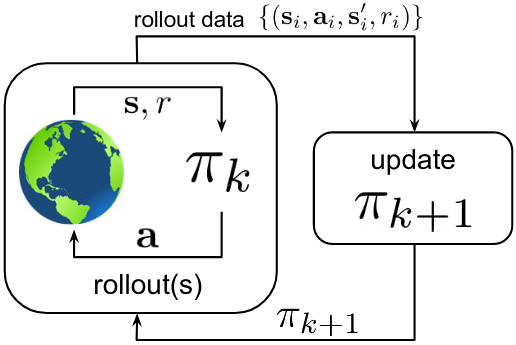
\includegraphics[width=5cm]{figures/on-policy.png}}
  \vspace{5mm} 
  
  \end{tabular}} &
  
  \multicolumn{2}{l|}{\begin{tabular}[c]{@{}l@{}}
  
Online, off-policy RL \\

  \raisebox{-\totalheight}{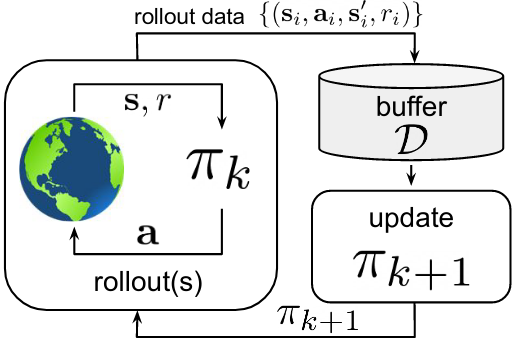
\includegraphics[width=5cm]{figures/off-policy.png}}
  \vspace{5mm} 
  
  \end{tabular}} \\ \hline
  
\multicolumn{1}{|p{3cm}|}{\textbf{Fixed dataset (no additional data collection)}} &
  \multicolumn{2}{c|}
  {-} 
  &
  \multicolumn{2}{l|}{\begin{tabular}[c]{@{}l@{}}
  
  Offline (fully off-policy) RL \\
  
  \raisebox{-\totalheight}{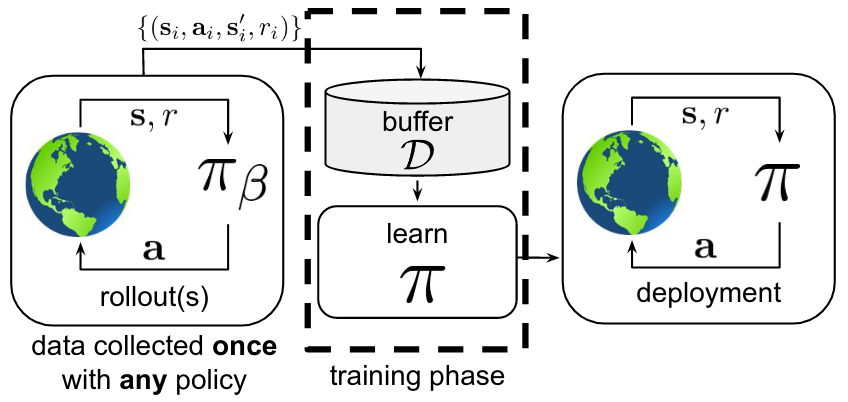
\includegraphics[width=7cm]{figures/offline.png}}
  
  \end{tabular}} \\ \hline
\end{tabular}
\caption{Classification of RL algorithms, \cite{Google_offline_RL}, \cite{youtube_offline_RL}
and \cite{Offline-RL-Levine:2020}.}
\label{tab:RL-classification}
\end{table}







\section{Function Approximation with Artificial Neural Networks}
\label{section:Function Approximation with Artificial Neural Networks}

The novel method presented in this thesis uses an artificial neural network (ANN) as a non-linear function approximator of the policy $\pi$ that the agent follows. ANNs are computational models inspired by biological neural systems and formed by interconnected processing elements. In particular, for this thesis, we will focus on fully-connected feedforward neural networks (FNN) where information flows in only one direction without going through any loop. In FNNs, the processing elements are called artificial neurons and they are arranged in consecutive structures called layers. There are three types of layers, the input layer, the hidden layer(s) and the output layer, see right of Figure \ref{fig:nn}. This hierarchy of layers makes it possible to model complex relationships among data as multiple levels of representation are learnt \cite{ANNs}.




An artificial neuron, see left of Figure \ref{fig:nn}, is the simplest element of an FNN. Similar to a biological neuron, an artificial neuron has input connections through which it receives external stimuli, the input data $x$ \cite{ANN-graupe:2013}. The neuron computes a weighted sum of the input data where the weights $w$ are the parameters of the model that have to be adjusted in order for the model to learn. Furthermore, there is an additional input connection to the neuron, the parameter bias $b$ that also is added to the weighted sum, $wx + b$. The final element of the artificial neuron is the activation function $f$ that takes the previous weighted sum as input and distorts it by adding non-linear deformations, $f(wx + b)$.



% ANNs can be classified according to multiple taxonomies, one of them refers to the direction in which the data is propagated through the layers. In particular, for this thesis, we will use feedworward neural networks (FNN) where information flows in only one direction from the input layer to the output layer without going through any loop.

  
  
  
   \begin{figure}[H]
  \centering
  \subfloat{{%
  \includesvg[width=.4\textwidth]{figures/neural_network.svg}}}
   \hfill
  \subfloat{{%
  \includesvg[width=.55\textwidth]{figures/neuron.svg}}}

  \caption{On the left, a simplification of the layers of fully-connected feedforward artificial neural network where all the neurons from one layer are connected to every neuron in the next layer. On the right, the main components of a single artificial neuron.}
  \label{fig:nn}
\end{figure}
















\section{Imitation Learning}
\label{section:Imitation Learning}

Imitation learning is a problem in machine learning where an agent learns a task leveraging the knowledge of a teacher which can be a human or a more experienced agent \cite{Imitation-Learning-definition-torabi:2019}. Imitation learning is more useful with respect to reinforcement learning when it is easier for a teacher to demonstrate or provide feedback in order for the agent to learn rather than to specify a reward function that would lead to the desired behaviour. The simplest imitation learning algorithm is called \textit{behavioural cloning} where a teacher provides some initial demonstrations and the agent tries to learn a policy via supervised learning.




\subsection{Interactive Imitation Learning}
\label{subsubsection:Interactive-Imitation-Learning}

% Interactive imitation learning is a branch of imitation learning \cite{lazydagger:2021}, where the teacher interacts with the agent \textit{during} its training providing feedback to improve its behaviour, see Figure \ref{fig:IIL}. The nature of the feedback varies between frameworks: Feedback in the form of evaluations (e.g., the TAMER framework \cite{TAMER-Knox-Stone:2009}) inform the agent how good or bad was the action taken. This kind of evaluative feedback is easier to implement than to define a reward function and allows a faster convergence than pure autonomous learning. However, the informativeness of this kind of evaluative feedback is still limited \cite{types-feedback-najar:2020}, and one way to improve it is to use corrections. 

% Feedback as relative corrections \cite{Relative-corrections-Celemin:2019} gives name to \textit{corrective imitation learning}, a branch of IIL which will be explained in detail in Section \ref{section:Correct Learning}. 


Interactive imitation learning (IIL) is a branch of imitation learning \cite{lazydagger:2021} where human teachers can help intelligent agents to learn \textit{during} their training, see Figure \ref{fig:IIL}. There are different forms in which the human can communicate his/her knowledge to facilitate the learning process. One way is for the human to demonstrate the task when the robot request it \cite{demonstration-robot-query} for example by teleoperating the robot or by using kinesthetic teaching. Another type of feedback are evaluations. Evaluative feedback in the form of scalar values (e.g., the framework Training an Agent Manually via Evaluative Reinforcement, TAMER \cite{TAMER-Knox-Stone:2009}) inform the agent how good or bad was the action taken. Evaluative feedback can also be provided as preferences between demonstrated trajectories \cite{learning-from-human-preferences:2018}. Here the human is presented with several executions of a policy, and he/she has to decide which one is better according to the goal of the task. Then, a reward function that explains the decisions of the human is found, and by applying RL, the agent learns how to perform the task. This kind of evaluative feedback is easier to implement than to define a reward function and allows a faster convergence than pure autonomous learning. However, the informativeness of this kind of evaluative feedback is still limited \cite{types-feedback-najar:2020}, and one way to improve it is to use corrections. 

Feedback as relative corrections (e.g., \cite{Relative-corrections-Celemin:2019}) gives name to \textit{corrective imitation learning (CIL)}, a branch of IIL. Corrective imitation learning improves the informativeness of evaluative feedback, by allowing the teacher to inform the agent whether the value of a taken action should be increased or decreased \cite{Relative-corrections-Celemin:2019} and it requires less exploration compared to evaluative feedback \cite{types-feedback-najar:2020}.


\subsection{On-Policy and Off-Policy Imitation Learning}
\label{subsubsection:on and off-policy Imitation Learning}

Subsection \ref{subsection:on and off-policy Reinforcement Learning} explained the meaning of the terms on-policy and off-policy in the field of reinforcement learning. When researching the literature it is clear that, for RL, the definition provided by Sutton and Barto in 1998 is the most used. However, things are not that obvious when talking about imitation learning. According to the paper \textit{An Algorithmic Perspective on Imitation Learning} \cite{Osa:2018} the first mention to the terms on-policy and off-policy regarding imitation learning is due to \cite{DBLP:journals/corr/LaskeyLHLMFG17}. These definitions are:
\setlength{\parskip}{1em} 

\say{In Off-Policy imitation learning, an agent observes demonstrations from a supervisor and tries to recover the behavior via supervised learning, an example of off-policy IL is behavioral cloning. On-policy imitation learning methods sample trajectories from the agent’s current distribution and update the model based on the data received. A common on-policy algorithm is DAgger.} 

\setlength{\parskip}{1em} 

Similar definitions are found in \cite{CSF-balakrishna:2020}:

\say{On-policy imitation learning involves executing the current agent's policy $\pi_{\theta_i}$ in the environment allowing it to make errors and observe new states and then soliciting feedback from a supervisor on the visited states to update $\pi_{\theta_i}$. This is in contrast to off-policy imitation learning algorithms where policy learning is performed entirely on states from the supervisor's trajectory distribution.}
 
\setlength{\parskip}{1em} 

% While we agree with the previous definition of on-policy IL, regarding off-policy IL, we consider that it is easier to interpret and relate its meaning to reinforcement learning, simply as the opposite of on-policy IL. Therefore our reinterpretation of the definitions is: 

% We consider that it is easier to interpret the terms and relate their meaning to reinforcement learning, simply as the opposite of on-policy IL. Therefore our reinterpretation of the definitions is:


We consider that it is necessary to redefine the terms on-policy IL and off-policy IL in order for their meaning to be closer to the well-accepted definitions in reinforcement learning. Therefore our reinterpretation of the definitions is:



\begin{itemize}
  \item \textbf{On-policy imitation learning}: \quotes{On-policy IL methods sample trajectories using the current agent’s policy and use that data to update that same policy.}
  
  \item \textbf{Off-policy imitation learning}: \quotes{Off-policy IL methods sample trajectories using any policy and use that data to update the current agent’s policy.}
  


\end{itemize}

For the case of off-policy imitation learning, \textit{any policy} could be a combination of different policies including the one of the agent, as it happens in off-policy RL.


In \cite{DBLP:journals/corr/LaskeyLHLMFG17}, \cite{OtherLaskeydefinitions:2019} and \cite{Osa:2018} the first example given for an on-policy imitation learning algorithm is DAgger (Dataset  Aggregation) \cite{DAgger-Ross:2011}. However, we consider important to make a clarification regarding this classification. The general principle of DAgger is to use a policy to collect a dataset at each iteration and then it trains the next policy under the aggregate of all collected datasets \cite{DAgger-Ross:2011}. The policy used to collect the dataset depends on whether it is the simple version or the general version of DAgger, both represented in Algorithm \ref{al:DAgger}. During the first iteration, both versions initialize the policy as the expert’s policy $\pi^*$ (line 2). The difference is that, for the next iterations, the general version implements a modified policy $\pi_i=\beta_i\pi^*+ (1−\beta_i)\hat{\pi}_i$ (line 8) to better leverage the knowledge of the expert. Depending on $\beta = [0,1]$, the expert policy $\pi^*$, is able to collect part of the next dataset by itself. If $\beta = 1$, the expert has full control when collecting the data, opposite to $\beta=0$  which means that all the data is gathered by the current agent's policy.
Therefore, we assume that the authors refer to the simple version of DAgger when classifying it as on-policy IL. But, even if referring to the simple version of DAgger, there is another reason to consider it off-policy. By its very nature, DAgger learns from a buffer, in other words, it learns from information gathered by older versions of the policy that are different from the current version.


% For the simple version, it initializes the policy For the first iteration, DAgger uses the expert’s policy $\pi^*$ (line 2), to collect a dataset of trajectories $D$ and then, it trains a policy  $\hat{\pi}_2$ that best mimics the expert on those trajectories. Then at iteration $n$, it uses $\hat{\pi}_n$ to collect more trajectories and adds those trajectories to the dataset $D$. The next policy $\hat{\pi}_{n+1}$ is the policy that best mimics the expert on the whole dataset $D$. 

% The authors of DAgger present two versions, a simple version and a more general version, both represented in in Algorithm \ref{al:DAgger}. 

% (line 5

% Algorithm \ref{al:DAgger} shows DAgger's \textit{simplest form}. For the first iteration, DAgger uses the expert’s policy $\pi^*$ (line 2), to collect a dataset of trajectories $D$ and then, it trains a policy  $\hat{\pi}_2$ that best mimics the expert on those trajectories. Then at iteration $n$, it uses $\hat{\pi}_n$ to collect more trajectories and adds those trajectories to the dataset $D$. The next policy $\hat{\pi}_{n+1}$ is the policy that best mimics the expert on the whole dataset $D$. In summary, DAgger uses its \textit{current policy} to collect a dataset at each iteration and trains the next policy under the aggregate of all collected datasets \cite{DAgger-Ross:2011}.


% However, and to better leverage the knowledge of the expert, the authors \textit{optionally} allow the algorithm to use a modified policy $\pi_i=\beta_i\pi^*+ (1−\beta_i)\hat{\pi}_i$. Depending on $\beta$,  which has values within the range $[0,1]$, the expert policy $\pi^*$, is able to collect part of the next dataset by itself. If $\beta = 1$, the expert has full control when collecting the data as is the case in Behavioural Cloning, opposite to $\beta=0$  which means that all the data is gathered by the current agent's policy. The parameter $\beta$ can be equal to $\beta_i=p^{i−1}$ representing a decaying rate over time of the usage of the expert to collect the data.

% This simple version of DAgger fits in the definition of on-policy imitation learning found in the literature because as can be seen in lines 4 and 5 of Algorithm \ref{al:DAgger-simplest}, the policy that gathers the trajectories is the current agent's policy.







% This more generic version represented in Algorithm \ref{al:DAgger-general} would not fit into the definition of on-policy imitation learning given by \cite{Osa:2018}, \cite{DBLP:journals/corr/LaskeyLHLMFG17}, \cite{OtherLaskeydefinitions:2019} and \cite{Anotherdefinitionfromberkeley:2020} because the expert's policy  intervenes in collecting the data.




\begin{algorithm}[H]
\caption{DAgger}
\begin{algorithmic}[1]
\State \textbf{Initialize} $\mathcal{D} \leftarrow 0$ 
\State \textbf{Initialize} $\hat{\pi}_1 \leftarrow \pi^*$ 
\For {$i = 1 $  \textbf{to} $N$} 

\If{Simple version of DAgger}
\State Let $\pi_i = \hat{\pi}_i$
\EndIf
\If{General version of DAgger}
\State Let $\pi_i = \beta_i\pi^* + (1 -\beta_i)\hat{\pi}_i$
\EndIf


\State Sample T-step trajectories using $\pi_i$
\State Get dataset  $\mathcal{D}_i = \{(s, \pi^*(s))\}$ of visited states by $\pi_i$ and actions given by expert
\State Aggregate datasets:  $\mathcal{D} \leftarrow \mathcal{D} \cup  \mathcal{D}_i$
\State  Train classifier $\hat{\pi}_{i+1}$ on $\mathcal{D}$
\EndFor
\State Return best $\hat{\pi}_i$ on validation
\end{algorithmic}
\label{al:DAgger}
\end{algorithm}



\subsection{Online and Offline Imitation Learning}
\label{subsubsection:online and offlineImitation Learning}
As it happens in RL, see Section \ref{subsection:Online and Offline}, imitation learning algorithms can also be classified as online or offline frameworks. In offline imitation learning, the agent learns by imitating a demonstrator without additional online environment interactions unlike in the case of online IL \cite{offlineIL}. This distinction between online and offline IL, which is similar to RL, justify our proposed definitions of on-policy IL and off-policy IL given that definitions for these terms found in the literature could be confused with the terms online and offline imitation learning.
% . The definitions on-policy and off-policy found in the literature could be confuse with the terms online and offline.


To conclude this subsection, we provide Table \ref{tab:classification_table} with a classification of several imitation learning algorithms according to the proposed definitions of the terms on-policy and off-policy IL as well as the terms online and offline IL. A list with a brief description of every method that appears in the table can be found in Annex \ref{appendix:List of Imitation Learning algorithms}.


\begin{table}[H]
\begin{tabular}{c|c|l|l|l|}
\cline{2-5}
\textbf{} &
  \multicolumn{2}{p{6.5cm}|}{\vspace{0.5mm} \textbf{On-policy Imitation Learning}\vspace{0.5mm}} &
  \multicolumn{2}{p{6.5cm}|}{\vspace{0.5mm}\textbf{Off-policy Imitation Learning}} \\ \hline
\multicolumn{1}{|p{1.8cm}|}{\textbf{Online IL}\vspace{0.5mm}} &

  \multicolumn{2}{p{6.5cm}|}{\begin{tabular}[c]{@{}l@{}}

  \vspace{1mm} \\
  TAMER \hspace{1mm} \cite{TAMER-Knox-Stone:2009}\\ 


  COACH \hspace{1mm}\cite{COACH-Celemin-Ruiz-del-Solar:2015}\\ 
  SHIV \hspace{1mm} \cite{SHIV-Laskey:2016}\\ 
  I-SABL \hspace{1mm}\cite{I-SABL-Loftin:2016}\\
  Convergent Actor-Critic by Humans \hspace{1mm}\cite{fakeCOACH-MacGlashan-Ho-Loftin:2017}\\
  Deep TAMER \hspace{1mm}\cite{DeepTAMER-Warnell-et-al:2018}\\ 
  D-COACH \hspace{1mm}\cite{D-COACH-Dattari-Celemin-Ruiz-del-Solar-Kober:2018}\\ 
  DQN-TAMER \hspace{1mm}\cite{DQN-TAMER-Arakawa:2018}\\
  LOKI \hspace{1mm}\cite{LOKI-Cheng:2018}\\
  AOR \hspace{1mm}\cite{OtherLaskeydefinitions:2019}\\
  ABLUF \hspace{1mm}\cite{ABLUF-he:2020}\\
  EIL \hspace{1mm}\cite{EIL-Spencer:2020}\\
    Learning from human preferences
  \cite{learning-from-human-preferences:2018}\\
\vspace{1mm} \\

  \end{tabular}} &
  
  
  
  
  \multicolumn{2}{l|}{\begin{tabular}[c]{@{}l@{}}
  \vspace{1mm} \\
  DAgger\hspace{1mm}\cite{DAgger-Ross:2011} \\
  DAgger by coaching \hspace{1mm} \cite{DAgger-by-coaching-He-DaumeIII-Eisner:2012}\\
  Advise \cite{Advise-Griffith-et-al:2013}\\
  AggreVaTe \hspace{1mm} \cite{AggreVaTe-Ross-Bagnell:2014}\\ 
  Safe DAgger \hspace{1mm} \cite{SafeDAgger-Zhang-Cho:2016}\\ 
  DropoutDAgger \hspace{1mm} \cite{DropoutDAgger}\\ 
  AggreVaTeD \hspace{1mm}\cite{AggreVaTeD-Sun:2017}\\
    Hierarchically Guided DAgger \hspace{1mm}\cite{Hierarchical-guidance-Le:2018}\\
  BAgger \hspace{1mm}\cite{BAgger-Cronrath:2018}\\ 
  Cycle of Learning \hspace{1mm}\cite{Cycle-of-Learning-waytowich:2018}\\
  Retrospective DAgger \hspace{1mm}\cite{Retrospective-DAgger-song:2019}\\ 
  SAIL \hspace{1mm}\cite{SAIL-Xiong:2019}\\
  HG-DAgger \hspace{1mm}\cite{HG-DAgger-Kelly:2019}\\
  EnsembleDAgger \hspace{1mm}\cite{EnsembleDAgger-Menda:2019}\\
  DAgger Replay Buffer \hspace{1mm}\cite{DA-RB-Prakash:2020}\\
  FRESH \hspace{1mm}\cite{FRESH-xiao:2020}\\
  FIRE \hspace{1mm}\cite{FIRE-ablett:2020}\\
  IWR \hspace{1mm}\cite{IWR-mandlekar:2020}\\
  ThriftyDAgger \hspace{1mm}\cite{ThriftyDAgger}

\vspace{1mm} \\





  
  
  \end{tabular}} \\ \hline
  
\multicolumn{1}{|p{1.8cm}|}{\textbf{Offline IL}} &
  \multicolumn{2}{c|}
  {-} 
  &
  \multicolumn{2}{l|}{\begin{tabular}[c]{@{}l@{}}
  \vspace{1mm} \\
  
  Behavioural Cloning \hspace{1mm}\cite{Behavioural-Cloning-Pomerleau:1991}\\ 
  DART \hspace{1mm}\cite{DART-Laskey:2017}\\ 
  ValueDICE \hspace{1mm}\cite{ValueDICE-Kostrikov:2019}\\
  SQIL \hspace{1mm}\cite{SQIL-Reddy-Dragan-Levine:2019}\\
%   Inverse Reinforcement Learning \hspace{1mm}\cite{inverse-reinforcement-learning}\\
  \vspace{1mm}
  \end{tabular}} \\ \hline
\end{tabular}
\caption{Classification of Imitation Learning algorithms}
\label{tab:classification_table}
\end{table}




\section{Corrective Imitation Learning}
\label{section:Corrective Imitation Learning}

As explained before, the goal of this master thesis is to develop a novel corrective imitation learning algorithm that is able to learn by replaying past corrections saved in a memory buffer. This process is very similar to the experience replay technique presented in Section \ref{subsection:Experience Replay} and to emphasise the fact that we are replaying corrections we refer to this technique as \textit{corrections replay} \cite{corrections-replay}.

The new framework that we propose in Chapter \ref{chapter:Proposed Method} is based on the D-COACH algorithm which, in turn, derives from the COACH algorithm; both methods are presented next.
% Section 4 concludes this review by explaining in detail the objective of this master thesis and the proposal to carry it out. 
% The goal is to transform the corrective imitation learning algorithm D-COACH, which is the deep version of the COACH algorithm, into an off-policy version that will incorporate an improved experience replay without the restrictions present in current version of D-COACH.







% In this Master Thesis we are going to focus on feedback in the form of relative corrections which is the type of feedback used in D-COACH \cite{D-COACH-Dattari-Celemin-Ruiz-del-Solar-Kober:2018}. The usage of corrective feedback names the term corrective imitation learning which we consider as a branch of IIL.


\subsection{COACH: Corrective Advice Communicated by Humans}
\label{subsection:COACH}

The method Corrective Advice Communicated by Humans, COACH \cite{COACH-Celemin-Ruiz-del-Solar:2015}, is a CIL framework designed for non-expert humans teachers where the person supervising the learning agent, provides occasional corrections when the agent behaves wrongly. This corrective feedback $h$ is a binary signal that indicates the direction in which the executed action $a = \pi_\theta(s)$, should be modified.
The parameters of the policy $\pi_\theta(s)$, $\theta$ are updated using a stochastic gradient descent (SGD) strategy in a supervised learning manner where the cost function $J(\theta)$ is the mean squared error between the applied and the desired action \cite{Gaussian-COACH-wout:2019}. Equation \eqref{eq:first-update-rule-D-COACH} shows the general update rule of the parameters $\theta$:


\begin{equation}
\theta \leftarrow \theta - \alpha \cdot \nabla_\theta J(\theta)
\label{eq:first-update-rule-D-COACH}
\end{equation}

COACH works under the assumption that teachers are non-experts and that therefore, they are just able to provide a correction trend that tells the sign of the policy error but not the error itself. To compute the exact magnitude of the error, COACH incorporates a hyperparameter $e$ that needs to be defined beforehand, resulting in $\text{error}_t = h_t \cdot e$  \cite{COACH-Celemin-Ruiz-del-Solar:2015}. The error needs to be defined as a function of the parameters in order to compute the gradient in the parameter space of the policy. Thus, the error can also be described as the difference between the desired action generated with the teacher's feedback, $a^\text{target}_t = a_t + \text{error}_t$ , and the current output of the policy, $a_t = \pi_\theta(o_t)$:


\begin{equation}
\text{error}_t(\theta) = a_t^\text{target} - a_t
\label{eq:error-D-COACH}
\end{equation}


Equation \eqref{eq:second-update-rule-D-COACH} shows the final update rule of COACH obtained from Equations \eqref{eq:first-update-rule-D-COACH}, \eqref{eq:error-D-COACH} and the derivative of the mean squared error:


\begin{equation}
\theta \leftarrow \theta + \alpha \cdot \text{error}_t \cdot \nabla_\theta \pi_\theta
\label{eq:second-update-rule-D-COACH}
\end{equation}



Where $\nabla_\theta \pi_\theta$ is the gradient of the policy, $\frac{\partial \pi}{\partial \theta}$, w.r.t the parameters $\theta$. Algorithm \ref{al:COACH} shows the pseudocode of the basic COACH version:


\begin{algorithm}[H]
\caption{Basic COACH}
\begin{algorithmic}[1]
\State $e \leftarrow \text{error magnitude}$ 
\State $\alpha \leftarrow \text{learning rate}$ 
\While {$\text{\textit{true}}$} {}
\State $s \leftarrow \text{getStateVec()}$
\State \textbf{execute} action $a_{t}=\pi_{\theta}(s_{t})$
\State \textbf{feedback} human corrective advice $h_{t}$
\If{$h_{t}$ is not \textbf{0}}
\State $\text{error}_{t} = h_{t}\cdot e$
\State $a_{\text{target}(t)} = a_{t} + \text{error}_{t}$
\State \textbf{update} $\pi$ using SGD with pair ($s_{t}$, $a^{\text{target}}_{t}$)
\EndIf
\EndWhile
\end{algorithmic}
\label{al:COACH}
\end{algorithm}

\subsection{D-COACH: Deep COACH}
\label{subsection:D-COACH}


Deep COACH, D-COACH \cite{D-COACH-Dattari-Celemin-Ruiz-del-Solar-Kober:2018}, is the \quotes{deep} version of the COACH algorithm in the sense that it uses an artificial neural network to represent the policy of the agent; Algorithm \ref{al:D-COACH} shows the pseudocode of D-COACH when learning from low-dimensional state space, and whose essence is very similar to COACH. The current version of D-COACH implements the corrections replay technique to be more data-efficient. During learning, tuples of old corrections, $(s_t, a^{\text{target}}_t)$, are stored in a memory buffer $\mathcal{B}$ and then they are replayed to update the current policy of the agent. However, the way that D-COACH implements the replaying of corrections has limitations. In this case, the replay buffer $\mathcal{B}$ works by assuming that \textit{recent} feedback is still being valid to update the most recent version of the policy. Due to this assumption, the size of the buffer that D-COACH implements, needs to be drastically reduced, otherwise old corrections could update the policy in undesired directions of the policy’s parameter space. On the other hand, a very small replay buffer will provoke an overfitting of the policy to data generated in the most recent trajectories, which limits the current version of D-COACH to work with low data intensive problems. It is necessary to mention that D-COACH \cite{D-COACH-Dattari-Celemin-Ruiz-del-Solar-Kober:2018} as well as  \cite{corrections-replay} and \cite{ResearchAssignmentpaper} which are based on D-COACH, employ state representation learning (SRL) strategies for learning a low-dimensional representation of the state, whose raw version consist on high-dimensional image states. This reduction of dimensionality makes the problem require less data and therefore it is easier to solve.




\begin{algorithm}[H]
\caption{Deep COACH}\label{algorithm:DeepCOACH}
\begin{algorithmic}[1]
\State \textbf{Require:} error magnitude $e$, buffer update interval $b$
\State \textbf{Init:} $\mathcal{B} = [\quad]$  \emph{\# initialize memory buffer}
\For{t = 1,2,...}{}
\State \textbf{observe} state $s_{t}$
\State \textbf{execute} action $a_{t}=\pi_{\theta}(s_{t})$
\State \textbf{feedback} human corrective advice $h_{t}$
\If{$h_{t}$ is not \textbf{0}}
\State $\text{error}_{t} = h_{t}\cdot e$
\State $a_{\text{target}(t)} = a_{t} + \text{error}_{t}$
\State \textbf{update} $\pi$ using SGD with pair ($s_{t}$, $a^{\text{target}}_{t}$)
\State \textbf{update} $\pi$ using SGD with a mini-batch sampled from $\mathcal{B}$
\State \textbf{append} $(s_{t}, a^{\text{target}}_{t})$ to $\mathcal{B}$
\EndIf
\If{mod(t, b) is 0 }
\State \textbf{update} $\pi_{\theta}$ using SGD with a mini-batch sampled from $\mathcal{B}$
\EndIf
\EndFor
\end{algorithmic}
\label{al:D-COACH}
\end{algorithm}


Figure \ref{fig:DCOACH_diagram} shows a graphical representation of the D-COACH algorithm. The red loop indicates a single update of the policy, which happens when the teacher provides a correction (line 10). On the other hand, the green loop represents a batch update in which by replaying corrections from the buffer, the policy is updated every time step that the teacher provides feedback (line 11) as well as every $b$ time steps (line 15).

\begin{figure}[H]
    \centering
    \adjustbox{trim=0cm 2.5cm 0cm 0cm}{%
  \includesvg[width=.84\textwidth]{figures/DCOACH-diagram.svg}}
    \caption{D-COACH agent}
    \label{fig:DCOACH_diagram}
\end{figure}


% However, it is important to remark that this replay buffer $\mathcal{B}$ is not completely correct; as it was mentioned in section \ref{sec:experience-replay}, ER techniques require an off-policy algorithm to work properly, but current D-COACH is on-policy because the policy is updated with data that depends on its most recent version. 




